\newpage
\section{Odometry Results}
\label{sec:odometry_results}

\begin{comment}
    Brief comment regarding odometry and connecting the work done to achieve this
\end{comment}

This section presents the result of the implemented pipeline as shown in Section~\ref{sec:processing_pipeline} with the dual-radar setup.
Two experimental environments were selected: a controlled laboratory environment and an outdoor scenario. 

\subsection{Laboratory Environment}
\subsubsection{Scenario Description}

The first experiments were conducted in an underground laboratory space (Fig.~\ref{fig:lab_setup}), which provided a controlled but reflective environment.  
The room contained multiple devices and metallic structures from other projects, which acted as additional landmarks.  

The main obstacle was created using a set of modular cushions arranged into a wall (black and orange blocks in Fig.~\ref{fig:lab_setup}).  
This configuration allowed us to test both straight-line odometry and more complex trajectories involving more complex set of trajectories.  

Three tests were performed:
\begin{itemize}
    \item \textbf{Straight-line test:} The vehicle was driven directly toward the cushion wall, covering a distance of approximately 10--11~m from the start point to the wall.  
    \item \textbf{Obstacle-avoidance test:} The vehicle followed a path around the cushion wall and returned to its starting location, introducing turning maneuvers that add stress to the tested system and additional opportunities for clutter-induced reflections. 
    \item \textbf{Hallway test:} The vehicle was pushed through the laboratoy hallway, which provides a highly reflective scenario in which a tight turn is possible to be tested.
\end{itemize}

\begin{figure}[!htbp]
    \centering
    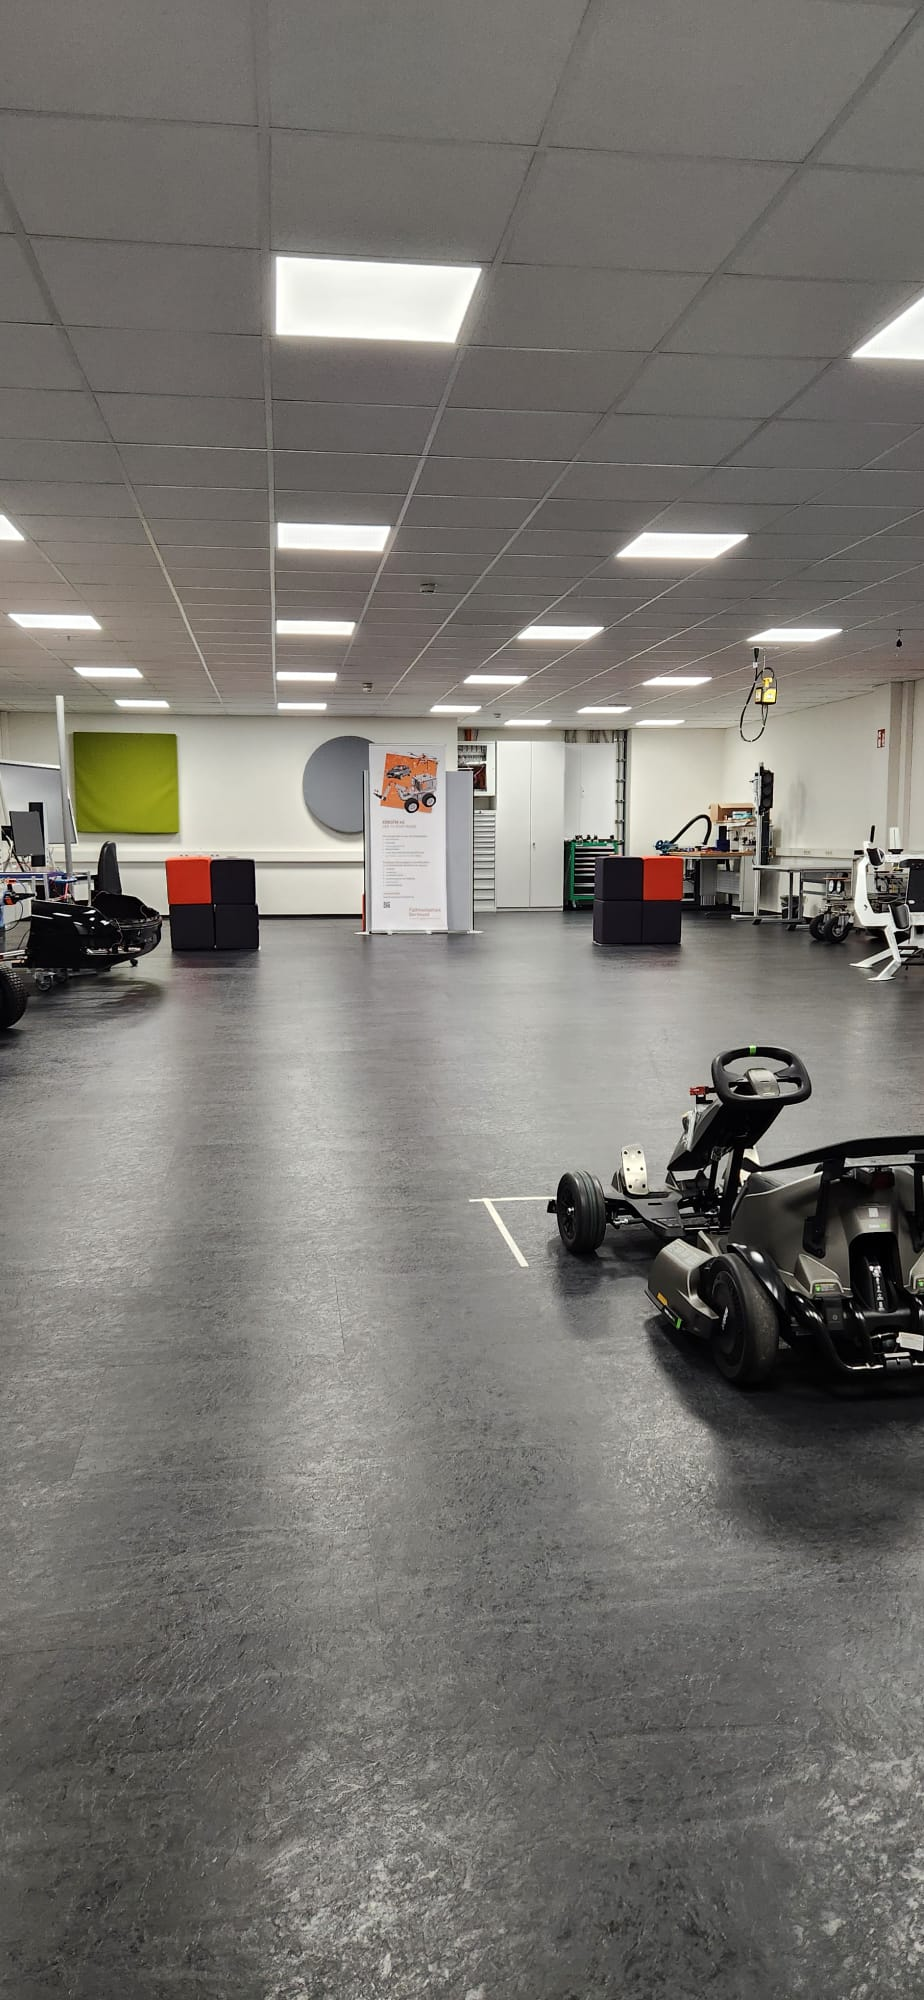
\includegraphics[width=0.75\linewidth]{images/labSetup.png}
    \caption{Laboratory environment setup. The cushion wall (black and orange) served as the main obstacle, while surrounding equipment contributed additional reflective surfaces.}
    \label{fig:lab_setup}
\end{figure}

\subsubsection{Odometry Results}
Two validation experiments were performed indoors to compare cluster-based ICP against full point cloud ICP.
Resulting trajectories from these are decribed where the test environment is shown in Fig.~\ref{fig:lab_setup}.

\begin{itemize}
    \item \textbf{Straight wall test, Fig.~\ref{fig:straightWall_Test}}:  
    In this scenario, the vehicle moved along a straight path of approximately 10~m.  
    This test provides the validation that the displacement measured by the odometry pipeline corresponds to the actual distance traveled, as there is no turns and can be described as the simplest of tests.  
    As shown in Fig.~\ref{fig:straightWall_FullICP}, the ICP alignment using the whole point-cloud produced a trajectory that closely matched the expected straight line.
    The cluster-based ICP failed in this case, measuring nearly double the actual distance.  
    The full point cloud ICP correctly reproduced the expected 10~m trajectory, confirming its reliability for straight-line validation. 
    
    \item \textbf{Drive-around (U-turn) test, Fig.~\ref{fig:labDriveAround}}:  
    In this scenario, a U-turn trajectory was performed to test the robustness of the pipeline in an enclosed environment with high reflections.  
    This test provided the opportunity for tight-turn tracking of the ego-motion estimation.  
    As shown in Fig.~\ref{fig:labDriveAroundFull}, ICP applied to the whole point cloud resulted in a more accurate ego-motion estimation.  
    The clustered ICP produced a trajectory not far from the true motion but showed reduced accuracy and consistency.  
    The total distance from the starting point to the wall being avoided was around 10~m.  

    \item \textbf{Hallway test, Fig.~\ref{fig:hallway_Test}}:  
    This experiment was performed in a narrow indoor hallway to evaluate the behavior of the system in a confined environment with strong multipath reflections.  
    Similar to the previous cases, both cluster-based and full point cloud ICP methods were applied.  
    As shown in Fig.~\ref{fig:hallway_Clustered}, the cluster-based ICP struggled to maintain consistent tracking due to limited visibility and varying reflections compared to Fig.~\ref{fig:hallway_Full}, resulting in a distorted trajectory.  
    In contrast, the full point cloud ICP produced a smoother and more reliable estimation of the path, confirming that in close or reflective environments, the full ICP approach remains superior.  

\end{itemize}

\begin{figure}[!htbp]
    \centering
    \begin{subfigure}{0.48\linewidth}
        \centering
        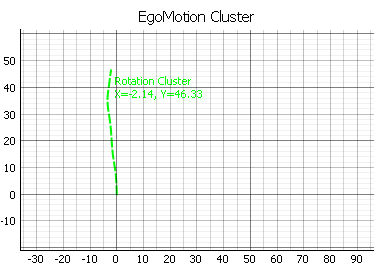
\includegraphics[width=\linewidth]{images/straightWallCluster_ICP.png}
        \caption{Cluster-based ICP alignment on the straight wall test.}
        \label{fig:straightWall_Clustered}
    \end{subfigure}
    \hfill
    \begin{subfigure}{0.48\linewidth}
        \centering
        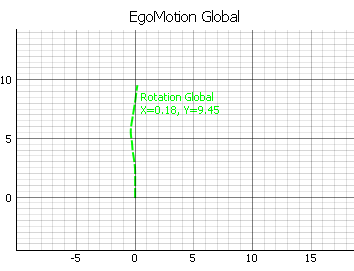
\includegraphics[width=\linewidth]{images/straightWallFull_ICP.png}
        \caption{Full point cloud ICP alignment on the straight wall test.}
        \label{fig:straightWall_FullICP}
    \end{subfigure}
    \caption{Straight wall validation test for odometry.  
    Both (a) cluster-based ICP and (b) full point cloud ICP were used to validate a previously measured distance, confirming correct functionality of the setup.}
    \label{fig:straightWall_Test}
\end{figure}

\begin{figure}[!htbp]
    \centering
    \begin{subfigure}{0.48\linewidth}
        \centering
        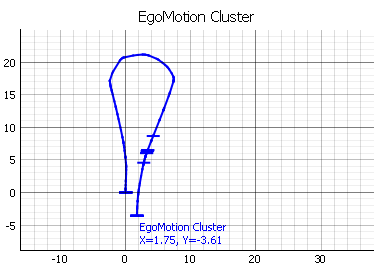
\includegraphics[width=\linewidth]{images/labDriveAroundICP_Cluster1.png}
        \caption{Cluster-based ICP trajectory for the laboratory U-turn test.}
        \label{fig:labDriveAroundClustered}
    \end{subfigure}
    \hfill
    \begin{subfigure}{0.48\linewidth}
        \centering
        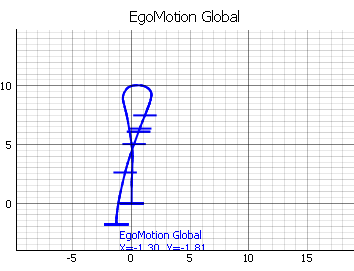
\includegraphics[width=\linewidth]{images/labDriveAroundICP_Full1.png}
        \caption{Full point cloud ICP trajectory for the same U-turn test.}
        \label{fig:labDriveAroundFull}
    \end{subfigure}
    \caption{Indoor U-turn test scenario: the vehicle avoids a target positioned approximately \SI{10}{\meter} from the starting point and stops slightly behind its initial position.  
    Comparison between (a) cluster-based ICP and (b) full point cloud ICP shows differences in trajectory accuracy under reflective indoor conditions.}
    \label{fig:labDriveAround}
\end{figure}

\begin{figure}[!htbp]
    \centering
    \begin{subfigure}{0.48\linewidth}
        \centering
        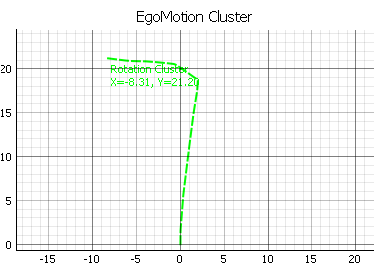
\includegraphics[width=\linewidth]{images/hallwayCluster_3.png}
        \caption{Cluster-based ICP trajectory in hallway test.}
        \label{fig:hallway_Clustered}
    \end{subfigure}
    \hfill
    \begin{subfigure}{0.48\linewidth}
        \centering
        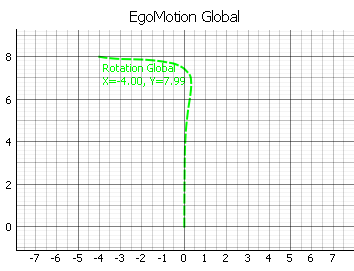
\includegraphics[width=\linewidth]{images/hallwayFull_3.png}
        \caption{Full point cloud ICP trajectory in hallway test.}
        \label{fig:hallway_Full}
    \end{subfigure}
    \caption{Hallway test scenario comparing (a) cluster-based ICP and (b) full point cloud ICP.  
    The confined environment and strong reflections increased uncertainty in the clustered approach, while the full point cloud ICP maintained a stable trajectory.}
    \label{fig:hallway_Test}
\end{figure}


\subsection{Outdoors Scenario}
\subsubsection{Scenario Description}
The second evaluation environment was the outdoor parking lot of Fachhochschule Dortmund (see Fig.~\ref{fig:parking_lot_overview}).  
The tests were conducted shortly after rainfall, which introduced additional radar clutter from wet ground reflections, making this a challenging stress test for the pipeline.  

The test area corresponds to a rectangular section of the parking lot, bounded by the building facades and a row of parked vehicles.  
Key dimensions were measured as shown in Fig.~\ref{fig:parkinglot_measurements}, with the vertical segment $L_1 \approx \SI{10.7}{\meter}$ and the horizontal segment $L_2 \approx \SI{54.1}{\meter}$.  
Combined, these form an L-shaped trajectory of approximately $\SI{62.3}{\meter}$ (Fig.~\ref{fig:parkinglot_totaldistance}).  

During the experiments, between 6 and 10 vehicles were parked in the area, providing strong reflective structures that contributed to odometry alignment.  

Two trajectories were tested:
\begin{itemize}
    \item \textbf{L-shape:} Starting along $L_2$, followed by a turn into $L_1$.
    \item \textbf{L-shape with return:} Same as above, but including a U-turn to return to the starting point.
\end{itemize}

All tests were driven exclusively in forward motion, as Doppler-based differentiation between forward and reverse trajectories was not implemented at this stage.

\begin{figure}[!htbp]
    \centering
    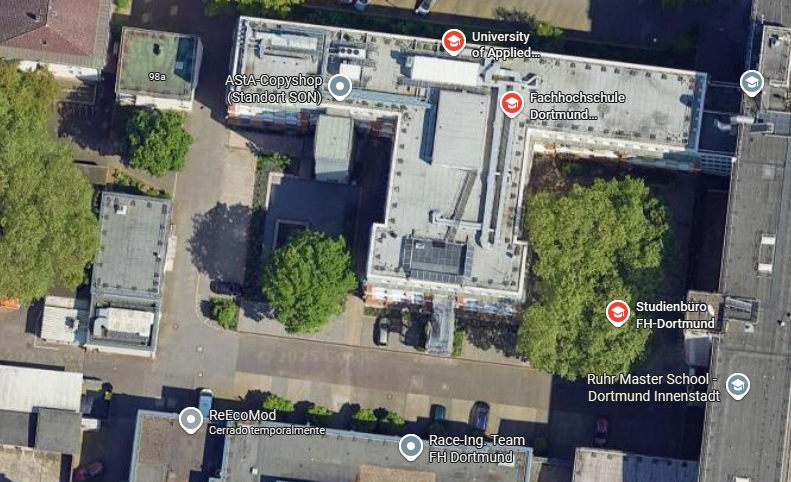
\includegraphics[width=0.9\linewidth]{images/FH_ParkingLot.png}
    \caption{Overview of the outdoor parking lot test environment at Fachhochschule Dortmund.\\
    \textit{Source: Google Maps, available at \url{https://maps.google.com} \cite{googlemaps_fhdo}}}
    \label{fig:parking_lot_overview}
\end{figure}

\begin{figure}[!htbp]
    \centering
    \begin{subfigure}{0.48\linewidth}
        \centering
        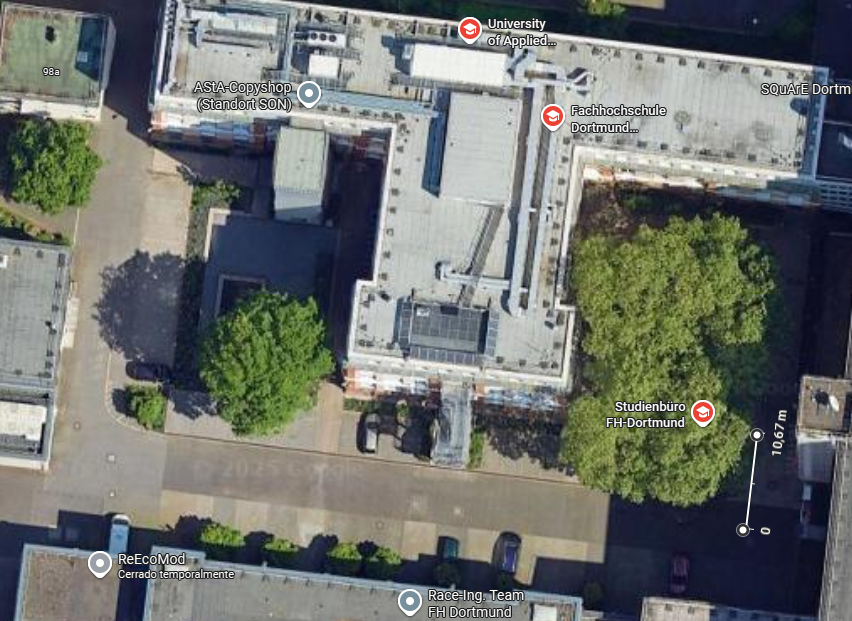
\includegraphics[width=\linewidth]{images/FH_ParkingLotL1.png}
        \caption{Vertical segment $L_1 \approx 10.7$ m.}
        \label{fig:parkinglot_l1}
    \end{subfigure}
    \hfill
    \begin{subfigure}{0.48\linewidth}
        \centering
        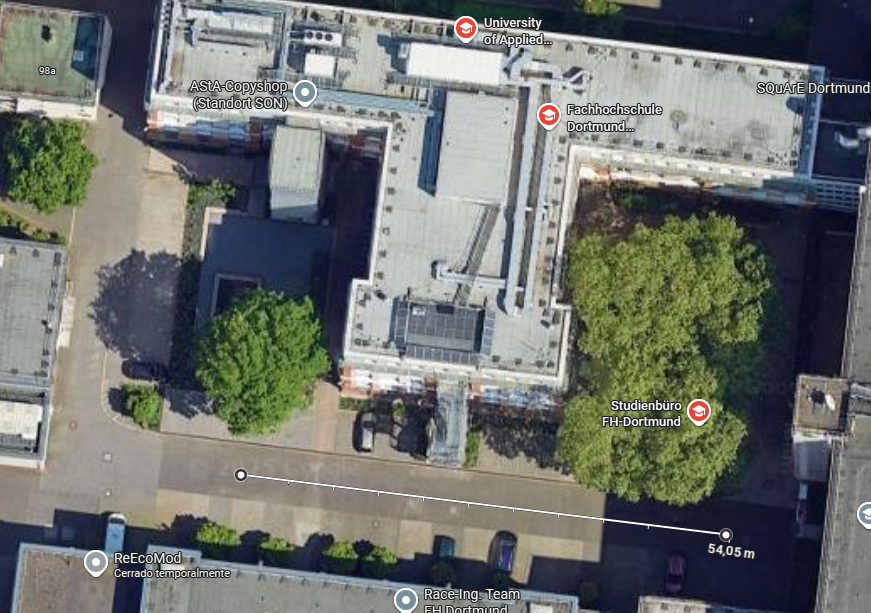
\includegraphics[width=\linewidth]{images/FH_ParkingLotL2.png}
        \caption{Horizontal segment $L_2 \approx 54.1$ m.}
        \label{fig:parkinglot_l2}
    \end{subfigure}
    \caption{Measured distances of the parking lot test area used for defining the L-shaped trajectory.\\
    \textit{Source: Google Maps, available at \url{https://maps.google.com} \cite{googlemaps_fhdo}}}
    \label{fig:parkinglot_measurements}
\end{figure}

\begin{figure}[!htbp]
    \centering
    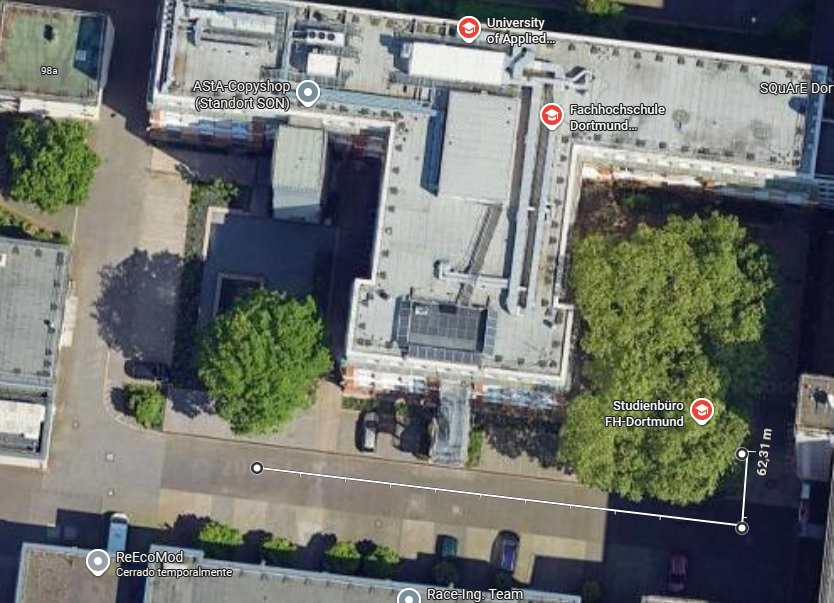
\includegraphics[width=0.9\linewidth]{images/FH_ParkingLot_TotalDistance.png}
    \caption{Combined L-shaped trajectory of approximately 62.3 m ($L_1 + L_2$).\\
    \textit{Source: Google Maps, available at \url{https://maps.google.com} \cite{googlemaps_fhdo}}}
    \label{fig:parkinglot_totaldistance}
\end{figure}

\subsubsection{Odometry Results}
Resulting trajectories from the recordings are shown from the outdoor tests in Fig.~\ref{fig:outsideOdometry4} and in Fig.~\ref{fig:outsideOdometry7}.
During this test the non idealistic weather allowed us to perform a perfect performance test for both of the solution in the outdoors environment.
In this testing period light rainfall was present, however nothing to damage the hardware.
In both scenarios an \textbf{L shape trajectory} was performed, however both where run at different lengths of the testing area.
As shown in Fig.~\ref{fig:outsideOdometry4}, the test was stoped around the metal emergency stair, which is around of 30 meters of the L1 section.
In Fig.~\ref{fig:outsideOdometry7} the full length was covered in which we get a pretty close estimation of the ego-motion of the vehicle converting this into a close estimation of the vehicle odometry.

\begin{comment}
    Add here the results of the odometry
\end{comment}

\begin{figure}[!htbp]
    \centering
    \begin{subfigure}{0.48\linewidth}
        \centering
        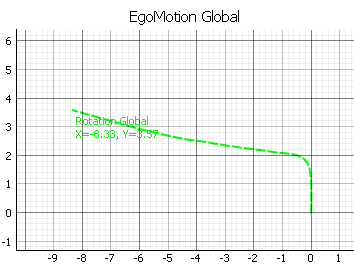
\includegraphics[width=\linewidth]{images/ICPOutside_Full4.png}
        \caption{Vehicle full point-cloud solution ICP ego-motion estimation. $L_1 \approx 10$ m., $L_2 \approx 30$ m. }
        \label{fig:odometryFull4}
    \end{subfigure}
    \hfill
    \begin{subfigure}{0.48\linewidth}
        \centering
        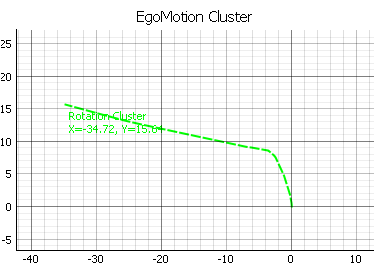
\includegraphics[width=\linewidth]{images/ICPOutside_Cluster4.png}
        \caption{Vehicle clustered solution ICP ego-motion estimation. $L_1 \approx 10$ m., $L_2 \approx 30$ m. }
        \label{fig:odometryCluster4}
    \end{subfigure}
    \caption{Outside test recording, reduced trajectory due to weather. $L_1 \approx 10$ m., $L_2 \approx 30$ m. }
    \label{fig:outsideOdometry4}
\end{figure}

\begin{figure}[!htbp]
    \centering
    \begin{subfigure}{0.48\linewidth}
        \centering
        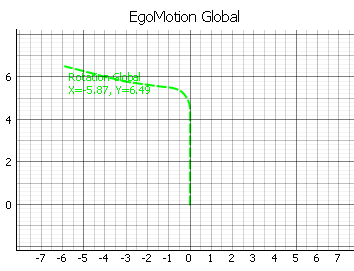
\includegraphics[width=\linewidth]{images/ICPOutside_Full7.png}
        \caption{Vehicle full point-cloud solution ICP ego-motion estimation. $L_1 \approx 10$ m., $L_2 \approx 60$ m. }
        \label{fig:odometryFull7}
    \end{subfigure}
    \hfill
    \begin{subfigure}{0.48\linewidth}
        \centering
        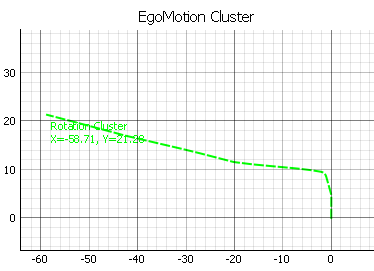
\includegraphics[width=\linewidth]{images/ICPOutside_Cluster7.png}
        \caption{Vehicle clustered solution ICP ego-motion estimation. $L_1 \approx 10$ m., $L_2 \approx 60$ m. }
        \label{fig:odometryCluster7}
    \end{subfigure}
    \caption{Outside test recording, full planned trajectory due to weather. $L_1 \approx 10$ m., $L_2 \approx 60$ m. }
    \label{fig:outsideOdometry7}
\end{figure}

\subsubsection{Observations}
The outdoor experiments highlighted the following:
\begin{itemize}
    \item Wet ground introduced additional clutter, especially near the dead zone as shown in Fig.~\ref{fig:outsideClutterRecording}, reinforcing the relevance of $y$-axis filtering.
    \item Parked vehicles provided strong static references that stabilized ICP alignment, particularly during turning maneuvers.
\end{itemize}

\begin{figure}[!htbp]
    \centering
    \begin{subfigure}{0.48\linewidth}
        \centering
        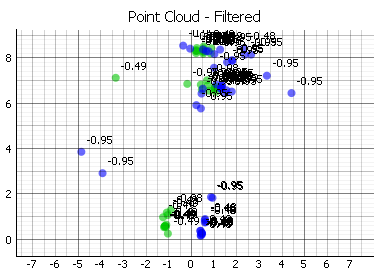
\includegraphics[width=\linewidth]{images/sensorClutterYAxisDualSensor.png}
        \caption{Full point-cloud of the observed clutter to aid the visualization of the whole point-cloud.}
        \label{fig:simpleClutter}
    \end{subfigure}
    \hfill
    \begin{subfigure}{0.48\linewidth}
        \centering
        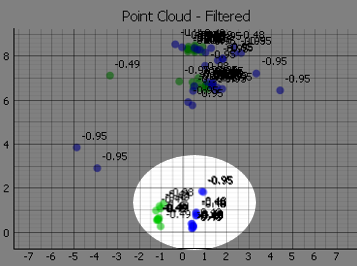
\includegraphics[width=\linewidth]{images/sensorClutterYAxisDualSensorHighlited.png}
        \caption{Highlighted clutter in the point-cloud to aid the visualization of the clutter.}
        \label{fig:highlightedClutter}
    \end{subfigure}
    \caption{Outside test recording, full planned trajectory due to weather. $L_1 \approx 10$ m., $L_2 \approx 60$ m. }
    \label{fig:outsideClutterRecording}
\end{figure}

Overall, the parking lot tests confirmed the pipeline's robustness in real-world outdoor conditions with environmental noise and complex reflectors, while also exposing drift-related challenges over extended distances.

\vspace{2\baselineskip}

\subsection{Discussion}
The two evaluation environments highlight different strengths and weaknesses of the proposed odometry pipeline.  

In the \textbf{laboratory environment}, performing ICP directly on the full point cloud delivered more stable results.  
The confined space, with multiple reflective surfaces and repeatable landmarks, produced a dense and consistent set of static detections.  
In this context, using all available points allowed ICP to maximize geometric alignment and minimize drift, even without the need for aggressive filtering of dynamic elements.  

In contrast, the \textbf{outdoor parking lot scenario} posed greater challenges.  
Non-ideal environmental conditions, such as recent rainfall, made this setting an effective stress test for the system.  
Sparse long-range detections and the presence of moving vehicles further contributed to a less consistent point cloud.  
Applying ICP on the entire point set in this environment led to instability and drift, as spurious or dynamic points distorted the alignment process.  
Instead, the clustered ICP approach—selecting the most consistent tracked cluster as the alignment reference—proved more effective.  
By anchoring to a reliable static object, the system achieved better trajectory consistency across extended distances.  

This comparison underlines a fundamental trade-off:
\begin{itemize}
    \item \textbf{Full point cloud ICP} excels in structured, controlled environments with dense and reliable landmarks.
    \item \textbf{Cluster-based ICP} provides robustness in unstructured or outdoor environments, where clutter and dynamics reduce the reliability of the full point cloud.
\end{itemize}

Although improvements are possible in both settings (e.g., more refined filtering, adaptive ICP weighting), the experiments suggest that cluster-based ICP is more suited for outdoor odometry, while full point cloud ICP can be leveraged indoors where landmark consistency is higher.
